\documentclass{beamer}
\usepackage{fancyvrb}
\usepackage{mathtools}
\usepackage{amsmath}
\usepackage{xcolor}
\usepackage{tikz}
\usepackage{graphicx}

\usetikzlibrary{calc}

\usecolortheme{rose}
\usefonttheme{structurebold}
\setbeamercovered{again covered=\opaqueness<1->{50}}
\setbeamertemplate{navigation symbols}{}

\newcommand{\highlight}[1]{%
  \colorbox{red!50}{$\displaystyle#1$}}

\newcommand{\beginner}{
  \begin{tikzpicture}[remember picture, overlay]
    \node at ($(current page.north east)+(-1cm,-1cm)$) {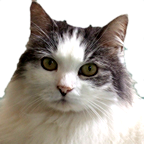
\includegraphics[width=1cm]{suzie.png}};
  \end{tikzpicture}
}

\title[pbkdf2]{PBKDF2: performance matters}
\author{Joseph Birr-Pixton\\
@jpixton\\
http://jbp.io/}
\date{}

\begin{document}

\frame{\titlepage}

\frame
{
  \begin{columns}[c]
    \column{.48\textwidth}
      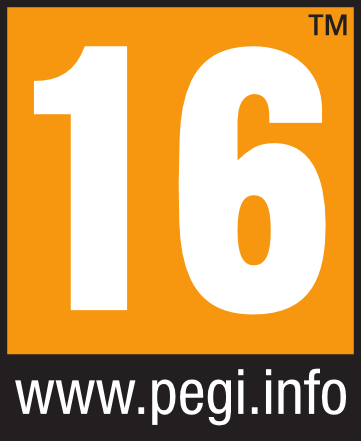
\includegraphics[width=4.7cm]{imgs/16years.png}\vspace{1mm}

      
\includegraphics[width=1.5cm]{imgs/anger.png}\hspace{1mm}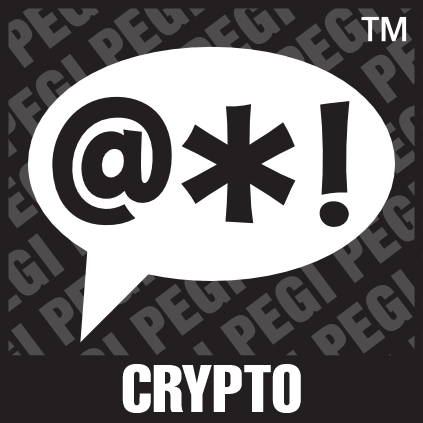
\includegraphics[width=1.5cm]{imgs/crypto.png}\hspace{1mm}
\includegraphics[width=1.5cm]{imgs/standards.png}
    \column{.48\textwidth}
      \begin{enumerate}
        \item<1> Quick intro to PBKDF2
        \item<2> The standard is bad
        \item<3> Your implementation is bad
        \item<4> A faster PBKDF2
      \end{enumerate}
  \end{columns}
}

\frame
{
  \frametitle{PBKDF2: quick intro} \beginner

  Purpose: deterministically and slowly derive a value from a password and salt.

  \begin{block}{Origin}<2>
    RSA labs, 1999. Described in PKCS\#5 and then RFC2898
  \end{block}
  
  \begin{block}{Usage}<3>
    \begin{itemize}
      \item Password verification (web sites, network services, etc.)
      \item Key derivation (disk encryption, key management, etc.)
    \end{itemize}
  \end{block}
}

\frame
{
  \frametitle{PBKDF2: quick intro} \beginner

  \begin{alertblock}{Performance}<1>
    Performance profile is \emph{important} for defenders.  Aim: to
    maximise attacker work for defender computation budget.
  \end{alertblock}

  \begin{exampleblock}{Simplification}<2>
    PBKDF2 can produce arbitrary length output.

    We're going to ignore this capability
    from here on in: only considering the first block of output.
    %\footnote{because it's broken, and complicates matters}
  \end{exampleblock}
}

\frame
{
  \frametitle{PBKDF2: how it was described} \beginner

  \begin{align*}
    \text{PBKDF2}_\text{PRF}(\text{pw}, \text{salt}, \text{i}) &\coloneqq U_1 \oplus U_2 \oplus \cdots \oplus U_\text{i} \\
    \onslide<2->{
      \text{where} \\
      U_1 &\coloneqq \text{PRF}(\text{pw}, \text{salt}\ \Vert\ 0_{32}) \\
      U_n &\coloneqq \text{PRF}(\text{pw}, U_{n-1}) \\
    }
    \onslide<3->{
      \text{and typically} \\
      \text{PRF}(\text{pw}, \text{x}) &= \text{HMAC-H}(\text{pw}, \text{x}) \\
      H &= \text{SHA-1, SHA-256, SHA-512, or ...}
    }
  \end{align*}
}

\frame
{
  \frametitle{Zoom, enhance} \beginner

  The function $\text{PBKDF2}_{\text{HMAC-SHA-256}}$ is slow because it
  executes the SHA-256 compression function many times.

  \begin{block}{How many times?}<2->
    Assumption: password and salt much shorter than SHA-256's 64-byte block size.
  \begin{align*}
    \text{HMAC-H}(key, msg) &\coloneqq
      \text{H}(\alert<5>{key \oplus \text{opad}}\ \Vert\ 
      \alert<6>{\text{H}(\alert<3>{key \oplus \text{ipad}}\ \Vert\ \alert<4>{msg})}) \\
    \onslide<3>{\text{block 1} &: key \oplus \text{ipad}} \\
    \onslide<4>{\text{block 2} &: msg} \\
    \onslide<5>{\text{block 3} &: key \oplus \text{opad}} \\
    \onslide<6>{\text{block 4} &: \text{block 2 output}}
  \end{align*}

  \uncover<7->{Therefore, we need to compute $4\text{i}$ SHA-256 blocks.}
  \end{block}
}

\frame
{
  \frametitle{Nope!}

  This is suboptimal.  Neither of the standards mention this, or
  even describe the expected performance :(

  \only<1>{\vspace{1cm}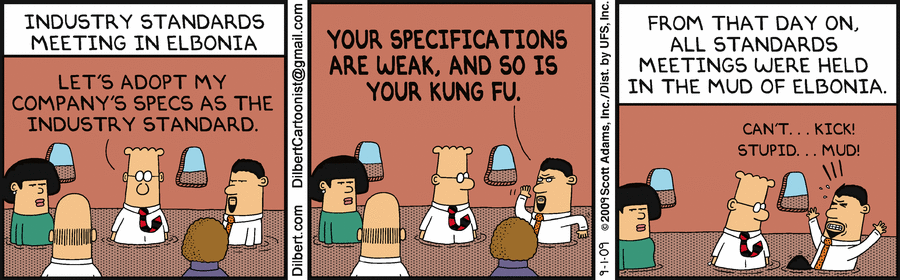
\includegraphics[width=11cm]{imgs/dilbert-2009-09-01.png}}

  \begin{align*}
    \onslide<2->{
    & U_1 \oplus U_2 \oplus \cdots \oplus U_\text{i} \\
    }
    \onslide<3->{
      \text{with} \\
      U_1 &\coloneqq \text{HMAC-H}(\text{pw}, \text{salt}\ \Vert\ 0_{32}) \\
      U_n &\coloneqq \text{HMAC-H}(\text{pw}, U_{n-1}) \\
    }
    \onslide<4->{
      \text{(or equivalently)} \\
      U_1 &\coloneqq \text{H}(\alert<5->{\text{pw} \oplus \text{opad}}\ \Vert\ \text{H}(\alert<5->{pw \oplus \text{ipad}}\ \Vert\ \text{salt}\ \Vert\ 0_{32})) \\
      U_n &\coloneqq \text{H}(\alert<5->{\text{pw} \oplus \text{opad}}\ \Vert\ \text{H}(\alert<5->{pw \oplus \text{ipad}}\ \Vert\ U_{n-1}))
    }
  \end{align*}

  \uncover<5->{We can compute these blocks once.}

  \begin{block}{How many times?}<6->
    Actually, we only need compute $2 + 2i$ SHA-256 blocks.
  \end{block}
}

\frame
{
  \frametitle{Survey of defender implementations}

  I looked at the following PBKDF2s:

  \begin{columns}[T]
    \column{.48\textwidth}
    \begin{itemize}
      \item FreeBSD 10
      \item GRUB 2.0
      \item Truecrypt 7.1a
      \item Android (disk encryption)
      \item Android (BouncyCastle)
      \item Django
      \item OpenSSL
      \item Python core ($\ge$3.4)
      \item Python (pypi pbkdf2)
      \item Ruby (pbkdf2 gem)
      \item Go (go.crypto)
    \end{itemize}
    \column{.48\textwidth}
    \begin{itemize}
      \item OpenBSD
      \item PolarSSL/mbedTLS
      \item CyaSSL/wolfSSL
      \item SJCL
      \item Java
      \item Common Lisp (ironclad)
      \item Perl (Crypt::PBKDF2)
      \item PHP5
      \item .NET framework
      \item scrypt/yescrypt\footnotemark
      \item BouncyCastle
    \end{itemize}
  \end{columns}
  
  \footnotetext[1]{never called for scrypt/yescrypt with iterations != 1}
}

\frame
{
  \frametitle{Our survey says...}

  \begin{columns}[T]
    \column{.48\textwidth}
    \begin{exampleblock}{Good: compute $2 + 2i$ blocks}
      \begin{itemize}
        \item SJCL
        \item<2-> OpenSSL (after Nov 2013)
        \item<2-> Python core ($\ge$3.4)
        \item<2-> Django (CVE-2013-1443, sc00bz)
        \item<2-> BouncyCastle ($\ge$1.49)
      \end{itemize}
    \end{exampleblock}
   
    \uncover<3->{
    \begin{alertblock}{Slow: compute $4i$ blocks}
      \begin{itemize}
        \item FreeBSD 10
        \item GRUB 2.0
        \item Android (BouncyCastle)
      \end{itemize}
    \end{alertblock}
    }

    \column{.48\textwidth}
    \uncover<4->{
    \begin{alertblock}{Slow: compute $4i$ blocks}
      \begin{itemize}
        \item Python (pypi pbkdf2)
        \item Ruby (pbkdf2 gem)
        \item Go (go.crypto)
        \item OpenBSD
        \item PolarSSL/mbedTLS
        \item CyaSSL/wolfSSL
        \item Java (OpenJDK)
        \item Common Lisp (ironclad)
        \item Perl (Crypt::PBKDF2)
        \item PHP
        \item .NET framework
        \item ...
      \end{itemize}
    \end{alertblock}
    }

  \end{columns}
}

\frame
{
  \frametitle{Selected performance measurements}

  \begin{itemize}
    \item<1> Question: how much practical difference does this make?
    \item<2> Let's measure PBKDF2-HMAC-SHA1 for large iteration count ($2^{22}$)
  \end{itemize}
}

\frame
{
  \frametitle{Selected performance measurements}

  \input measurements.tex

  \begin{figure}
  \centering

  \begin{tikzpicture}[
    y = .25cm,
    x = .7cm,
    font = \small\sffamily,
    fast/.style = {circle, draw=green!50, fill=green!20, thick, inner sep=0.8mm, outer sep=1mm},
    maybefast/.style = {circle, draw=green!25, fill=green!10, thick, inner sep=0.8mm, outer sep=1mm},
    slow/.style = {circle, draw=red!50, fill=red!20, thick, inner sep=0.8mm, outer sep=1mm},
    thing/.style = {font=\footnotesize},
    maybe/.style = {draw=black!50},
  ]
    \draw (0,0) -- coordinate (y axis mid) (0,22);
    \draw (0,0) -- (14,0);
    \foreach \y in {0,2,...,22} {
      \draw (0pt,\y) -- (-3pt,\y) node[anchor=east] {\y};
      \draw (0,\y) -- (14,\y) [gray!30];
    }
    \foreach \y in {1,3,...,21} {
      \draw (0pt,\y) -- (-1pt,\y);
    }
    \node[rotate=90, above=0.8cm] at (y axis mid) {Seconds};

    \node[fast,label=right:\openssltime] at (1,\openssltime) {};
    \node[thing] at (1,-1) {OpenSSL};

    \uncover<2-> {
    \node[fast,label=right:\pythontime] at (3,\pythontime) {};
    \node[thing] at (3,-2) {Python 3.4};
    % all openssl/openssl-derived
    }

    \uncover<3-> {
    \node[slow,label=right:\phptime] (php) at (5,\phptime) {};
    \node[thing] at (5,-1) {PHP5};

    \node[slow,label=right:\javaopenjdktime] (java) at (7,\javaopenjdktime) {};
    \node[thing] at (7,-2) {Java};

    \node[slow,label=right:\golangtime] (golang) at (9,\golangtime) {};
    \node[thing] at (9,-1) {Go};
    }

    \visible<4-5> {
    \node[fast,label=right:\phppatchtime] (phppatch) at (5,\phppatchtime) {};
    \draw [->] (php) -- (phppatch);
    % pull req https://github.com/php/php-src/pull/1387
    }

    \visible<5> {
    \node[maybefast,label=right:?] (javamaybefast) at (7,\javaopenjdktime*\phppatchtime/\phptime) {};
    \draw [maybe,->] (java) -- (javamaybefast);

    \node[maybefast,label=right:?] (golangmaybefast) at (9,\golangtime*\phppatchtime/\phptime) {};
    \draw [maybe,->] (golang) -- (golangmaybefast);
    }

    \uncover<6-> {
    \node[fast,label=right:\fastpbkdftime] at (11,\fastpbkdftime) {};
    \node[thing] at (11,-2) {fastpbkdf2};
    }

  \end{tikzpicture}
  
  \caption{PBKDF2-HMAC-SHA1, one block output, $2^{22}$ iterations}
  \end{figure}

}

\frame
{
  \frametitle{fastpbkdf2}

  A faster PBKDF2-HMAC-\{SHA-1,SHA-256,SHA-512\} for defenders.

  \begin{itemize}
    \item<1-> About 400 lines of C99.
    \item<2-> Uses OpenSSL libcrypto's hash functions.
    \item<3-> CC0.
    \item<4-> https://github.com/ctz/fastpbkdf2/
  \end{itemize}
}

\frame
{
  \frametitle{Parting thoughts...}

  \begin{itemize}
    \item<1-> PBKDF2 is a poor design, and described in an unhelpful way by its authors.
    \item<2-> Most implementations waste time and power.
    \item<3-> If you use PBKDF2, you can probably drop in a faster implementation\only<3>{.}
              \only<4>{and either
              increase security margin, or improve time/power performance.}
    \item<4-> Please try not to use PBKDF2 any more.
  \end{itemize}
}

\frame
{
  \frametitle{Thank you!}
  Questions?

  \vspace{5em}

  Twitter: @jpixton

  Mail: jbp@jbp.io

  Web: https://jbp.io/

  Slides and benchmarking code: https://github.com/ctz/talks/
}

\end{document}
